\documentclass[12pt]{article}
\usepackage[utf8]{inputenc}
\usepackage[english,russian]{babel}
\usepackage{graphicx}
\usepackage{amsmath}
\usepackage{amsthm}
\usepackage{caption}
\usepackage{tikz}
\usepackage{subcaption}
\usepackage{imakeidx}
\usepackage[russian]{cleveref}
\usepackage[a4paper,left=15mm,right=15mm,top=30mm,bottom=20mm]{geometry}
\parindent=0mm
\parskip=3mm

\makeindex
\pagestyle{empty}

\title{ДЗ 0, Дискретная Математика}
\author{Егор Богомолов}
\date{03.09.2019}

\begin{document}

\maketitle

\begin{enumerate}
\item % Задание 1
Короткое и красивое решение первого задания. Так выглядят формулы в тексте $A_k$. Больше информации про формулы можно найти в интернете\footnote{Например: https://www.latex-tutorial.com/tutorials/amsmath/} или спросить.

Большие формулы пишем вне текста, вот так:
$$
|A'\cap B'|=|(A\cup B)'|=|X|-|A\cup B|=|X|-|A|-|B|+|A\cap B|
$$
$$
\sum\limits_{k=1}^{n} \binom{n}{k} \cdot A_k^{n+1}
$$

\item % Задание 2
Длинное и некрасивое решение второго задания, зато с картинкой.

\begin{figure}[h]
\centering
 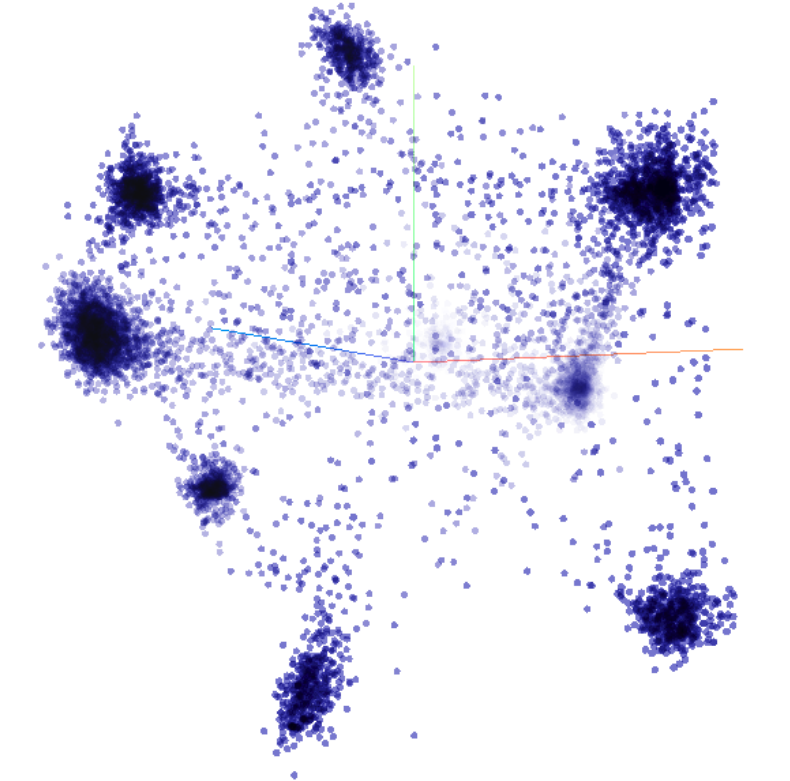
\includegraphics[width=0.5\linewidth]{figures/picture-01.png}
 \caption{Какие-то синие векторы}
 \label{fig:vectors}
\end{figure}

В тексте на картинку можно сослаться вот так: смотри \cref{fig:vectors}. Изменить ее размер можно поменяв множитель перед linewidth.

\item % Задание 3
\item % Задание 4
Для нерешенных заданий (3 в данном случае) оставляйте пустой item.

Если будут возникать какие-то вопросы про tex, то не стесняйтесь писать.
Обратите внимание, что строка переносится в тексте ДВУМЯ пустыми строками в исходном файле.
\end{enumerate}

\end{document}